% !TeX spellcheck = en_US
\section{Problem 7}
Modeling expressions as fuzzy subsets in the context of fuzzy logic allows us to handle the uncertainty and imprecision inherent in certain descriptions like \say{large}, \say{very small}, or \say{medium-weight}. In fuzzy logic, each element of the subset has a degree of membership ranging from 0 to 1, where 0 means \say{not a member at all} and 1 means \say{fully a member}.\\
Below are examples of how you might model the given expressions as fuzzy subsets using MATLAB code snippets, assuming some reasonable definitions for each term.\\

\underline{LARGE INTEGERS}\\
For \say{Large integers}, we need a membership function that gradually increases as the integers become larger. A simple way to model this is to use a function that increases the membership score as the number exceeds a certain threshold. However, defining \say{large} is subjective and can vary depending on the context. For simplicity, let's assume integers greater than 100 are considered large, but the transition starts at 50, becoming more \say{large} as the number increases.

\begin{figure}[h]
	\centering
	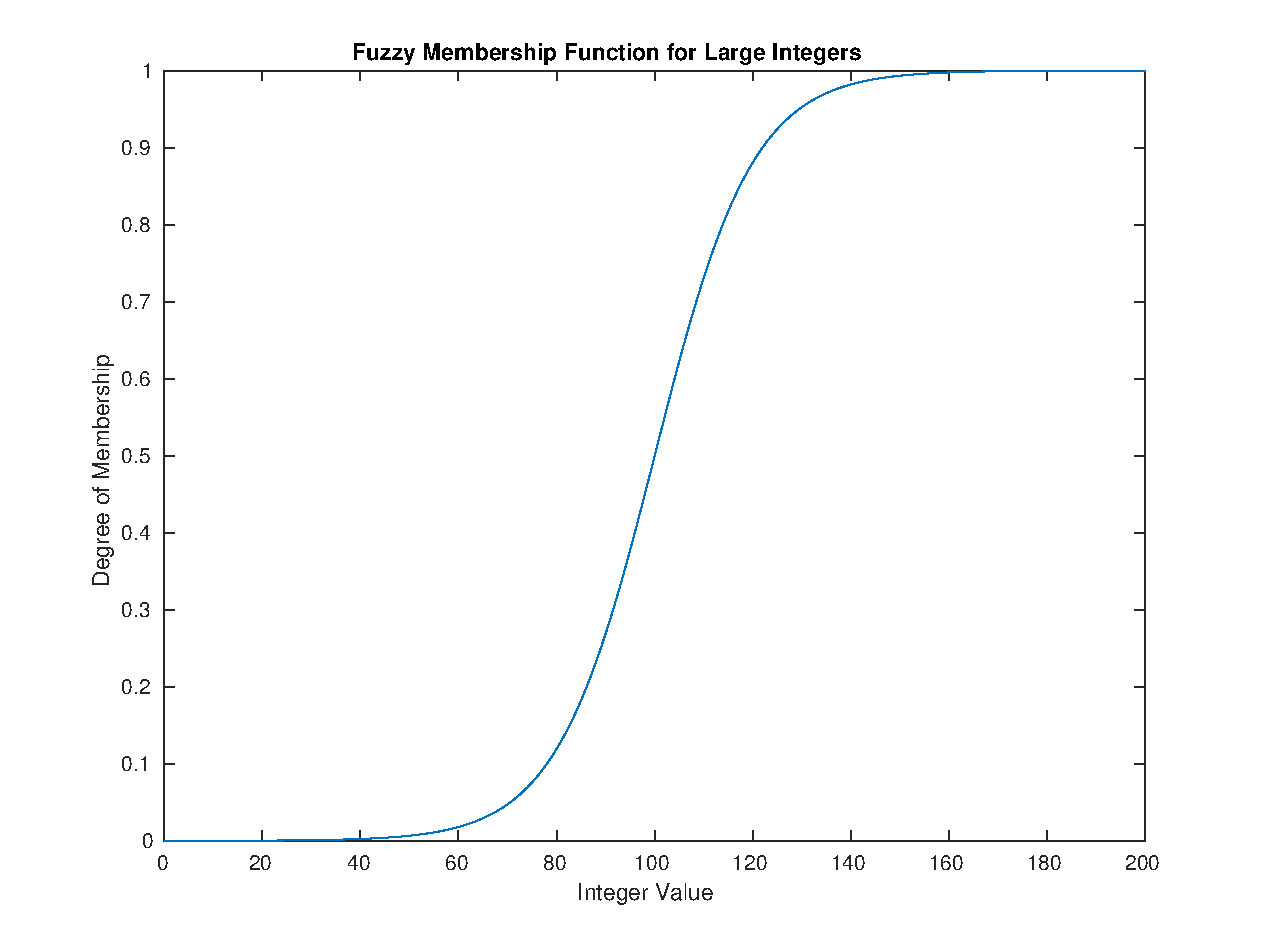
\includegraphics[width=0.6\textwidth]{../Problem 7/large_int.pdf}
	\caption{Fuzzy membership function for Large Integers}	
\end{figure}
we are using the sigmoid function for a smooth transition.
\vspace{5mm}

\underline{VERY SMALL NUMBERS}\\
For \say{very small numbers}, we can consider numbers close to zero as having a higher degree of membership. \say{Very small numbers} can include both positive numbers close to zero and negative numbers. For this, a membership function that assigns higher scores to numbers closer to zero can be used. We'll focus on positive numbers for simplicity, but this can be adjusted to include negatives.

\begin{figure}[H]
	\centering
	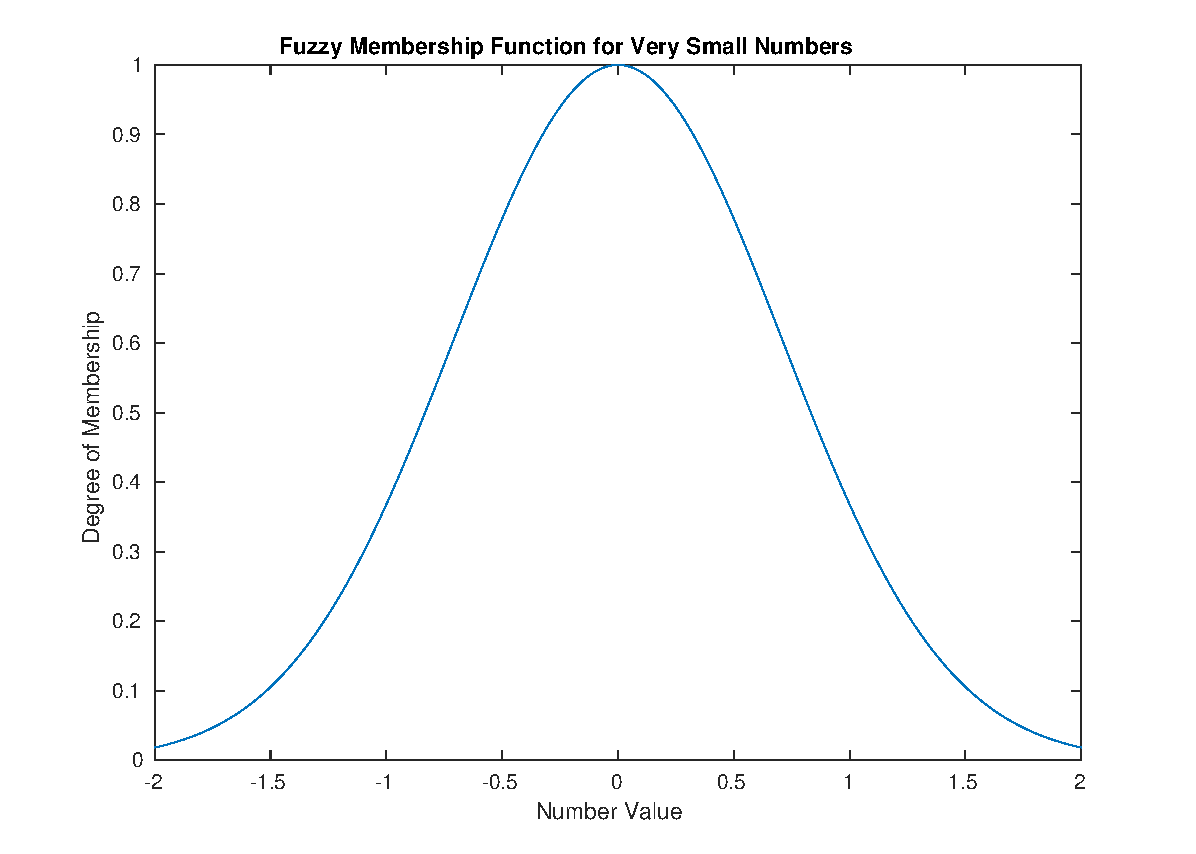
\includegraphics[width=0.6\textwidth]{../Problem 7/small_int.pdf}
	\caption{Fuzzy membership function for Very Small Numbers}	
\end{figure}
we are using the Gaussian function centered at 0.
\vspace{5mm}

\underline{MEDIUM-WEIGHT MEN}\\
Assuming the average weight range for medium-weight men is between 70kg and 90kg, with the peak at 75kg, we used another Gaussian function centered around 75kg, considering an average weight range. This function assigns a higher degree of membership to weights close to 75kg, with the membership degree decreasing for weights further away from this center. This approach models the fuzzy concept of \say{medium weight}.

\begin{figure}[H]
	\centering
	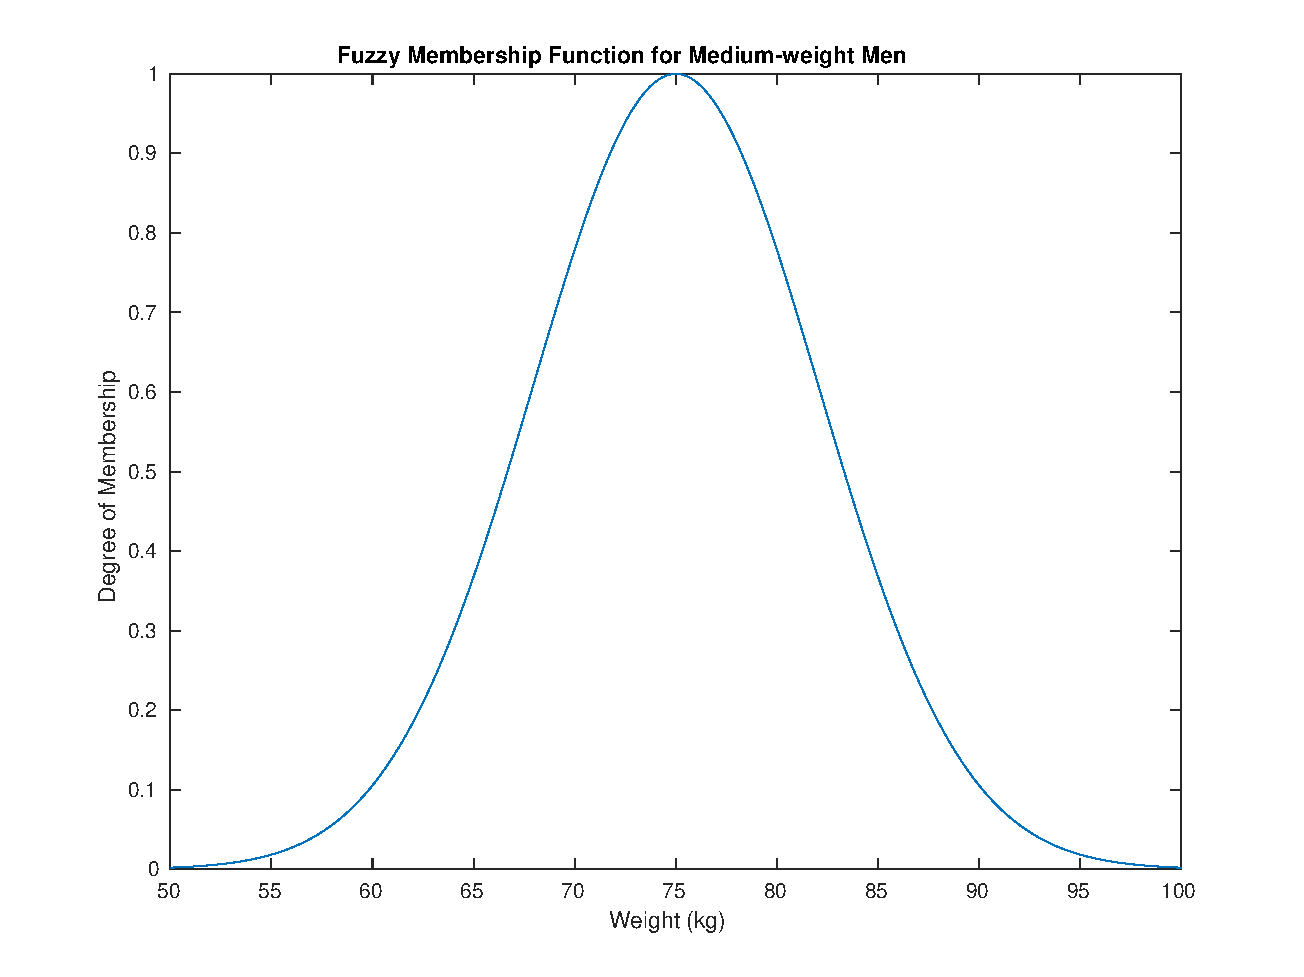
\includegraphics[width=0.6\textwidth]{../Problem 7/medium_weight.pdf}
	\caption{Fuzzy membership function for Medium\_weighted Men}	
\end{figure}
\vspace{5mm}

\underline{NUMBEES APPROXIMATELY BETWEEN 10-20}\\
For numbers approximately between 10 and 20, a trapezoidal membership function is employed to model numbers in this range, providing a clear illustration of numbers with a high degree of membership strictly within the 10 to 20 range, and a linear decrease to 0 as numbers diverge from this range. This function effectively captures the fuzzy boundaries of being \say{approximately between} two values.

\begin{figure}[H]
	\centering
	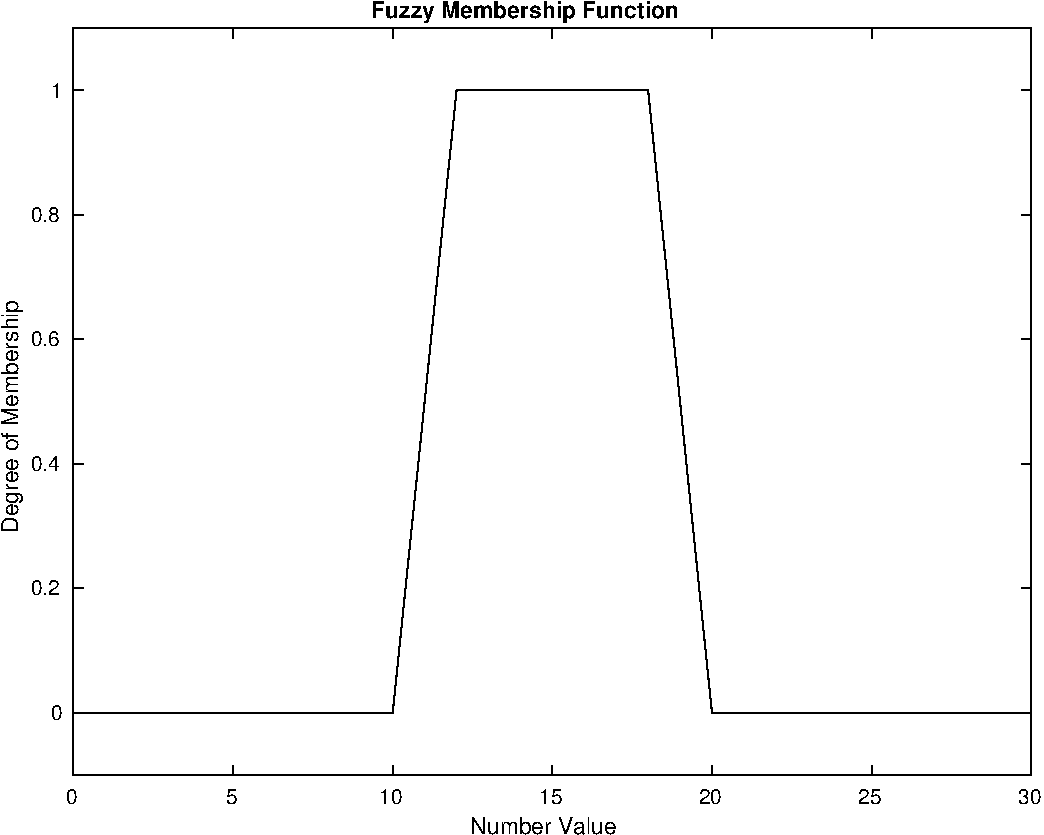
\includegraphics[width=0.6\textwidth]{../Problem 7/number_range.pdf}
	\caption{Fuzzy membership function for Numbers approximately between 10 and 20}	
\end{figure}
\vspace{5mm}

To summarize, modeling expressions as fuzzy subsets involves assigning a degree of membership to each element relative to a particular set based on its characteristics. 
In fuzzy logic, the choice of membership function (such as sigmoid, Gaussian, or trapezoidal) depends on the specific context and the nature of the fuzzy set being modeled. These functions help in translating vague or imprecise terms into a quantitative framework that can be analyzed and manipulated mathematically.